
\chapter{PENDAHULUAN}

\section{Latar Belakang}
\blindtext

\begin{afigure}{Sebuah gambar}
    \label{fig:figure2}
    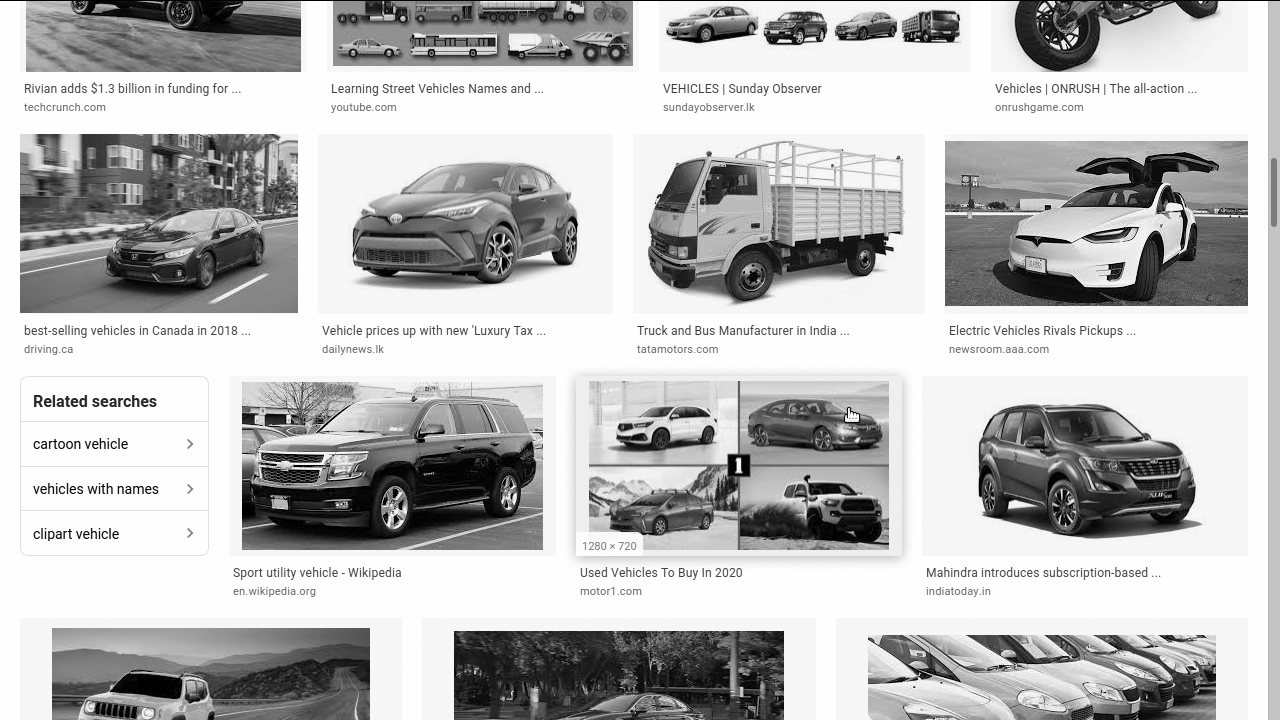
\includegraphics[width=0.5\textwidth, center]{images/input.png}
\end{afigure}

\blindtext

\section{Rumusan Masalah}
\blindtext

\begin{atable}{Ini Caption tabel}
    \label{table:tabl}
    \begin{tabular}{|l|l|l|l|l|}
    \hline
    fad  & dfaf & fdsfdfads & fdasf & fda  \\
    \hline
    fdas & fdas & ss        & ss    & ss   \\
    \hline
    ss   & dfa  & dfsa      & fdsa  & fdsa \\
    \hline
    ddd  & fdd  & dda       & da    & da \\
    \hline
    \end{tabular}
\end{atable}

\blindtext
~\ref{fig:figure2}
\\
for reference ~\ref{table:tabl}

\begin{afigure}{ini gambar na}
    \label{fig:f1}
    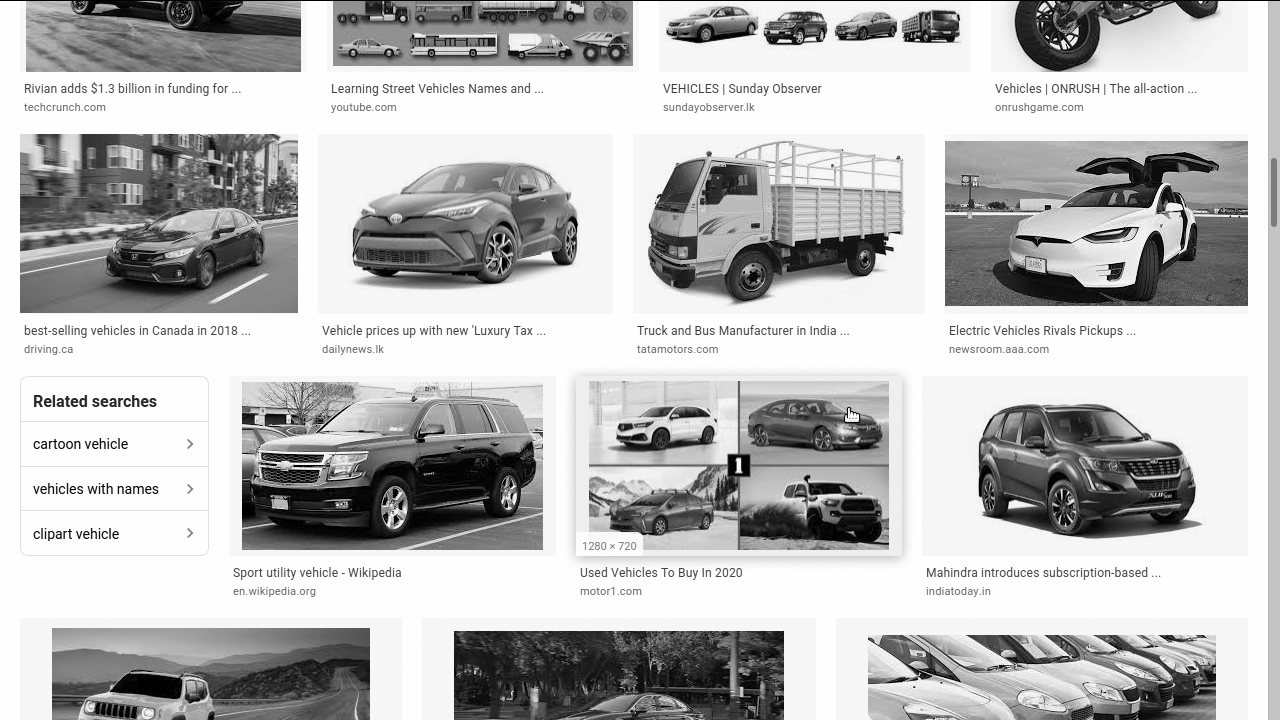
\includegraphics[width=0.5\textwidth, center]{images/input.png}
\end{afigure}
